\subsection{Design}


\subsubsection{Scenarios}

Since milestone 3 VFS Browser can run in three different modes. Classic
mode\ref{fig:scenario_classic_mode} basically is the usage of virtual disks without any
server involved. Online mode\ref{fig:scenario_online_mode} allows immediate
propagation of changes to the server, which propagates them to other clients.
Offline mode\ref{fig:scenario_offline_mode} allows the offline VFS Browser to
make changes to a local disk (step 1). In this mode
changes are recorded in a journal. When the VFS Browser later on connects the
the server the journal is sent to the server which applies the changes to its 
own disk copies and propagates the journal to the other attached clients. In
this step possible changes on the server side are sent to the freshly attached
client. 

\begin{figure}[h!]
\centering
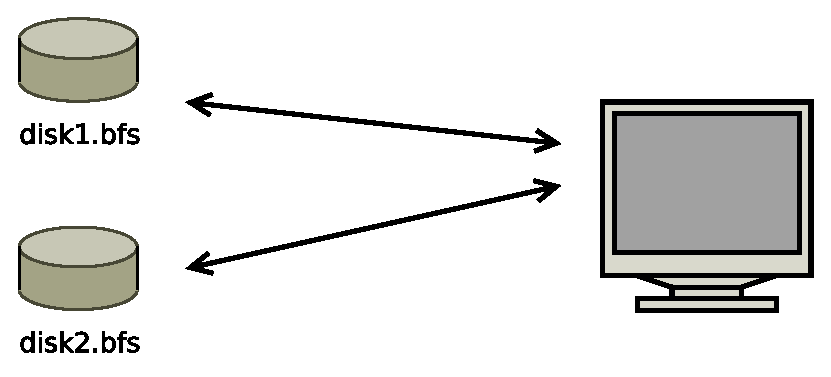
\includegraphics[width=1\textwidth]{figures/scenario_classic_mode.eps}
\caption{scenario classic mode}
\label{fig:scenario_classic_mode}
\end{figure}

\paragraph{online mode}

\begin{figure}[h!]
\centering
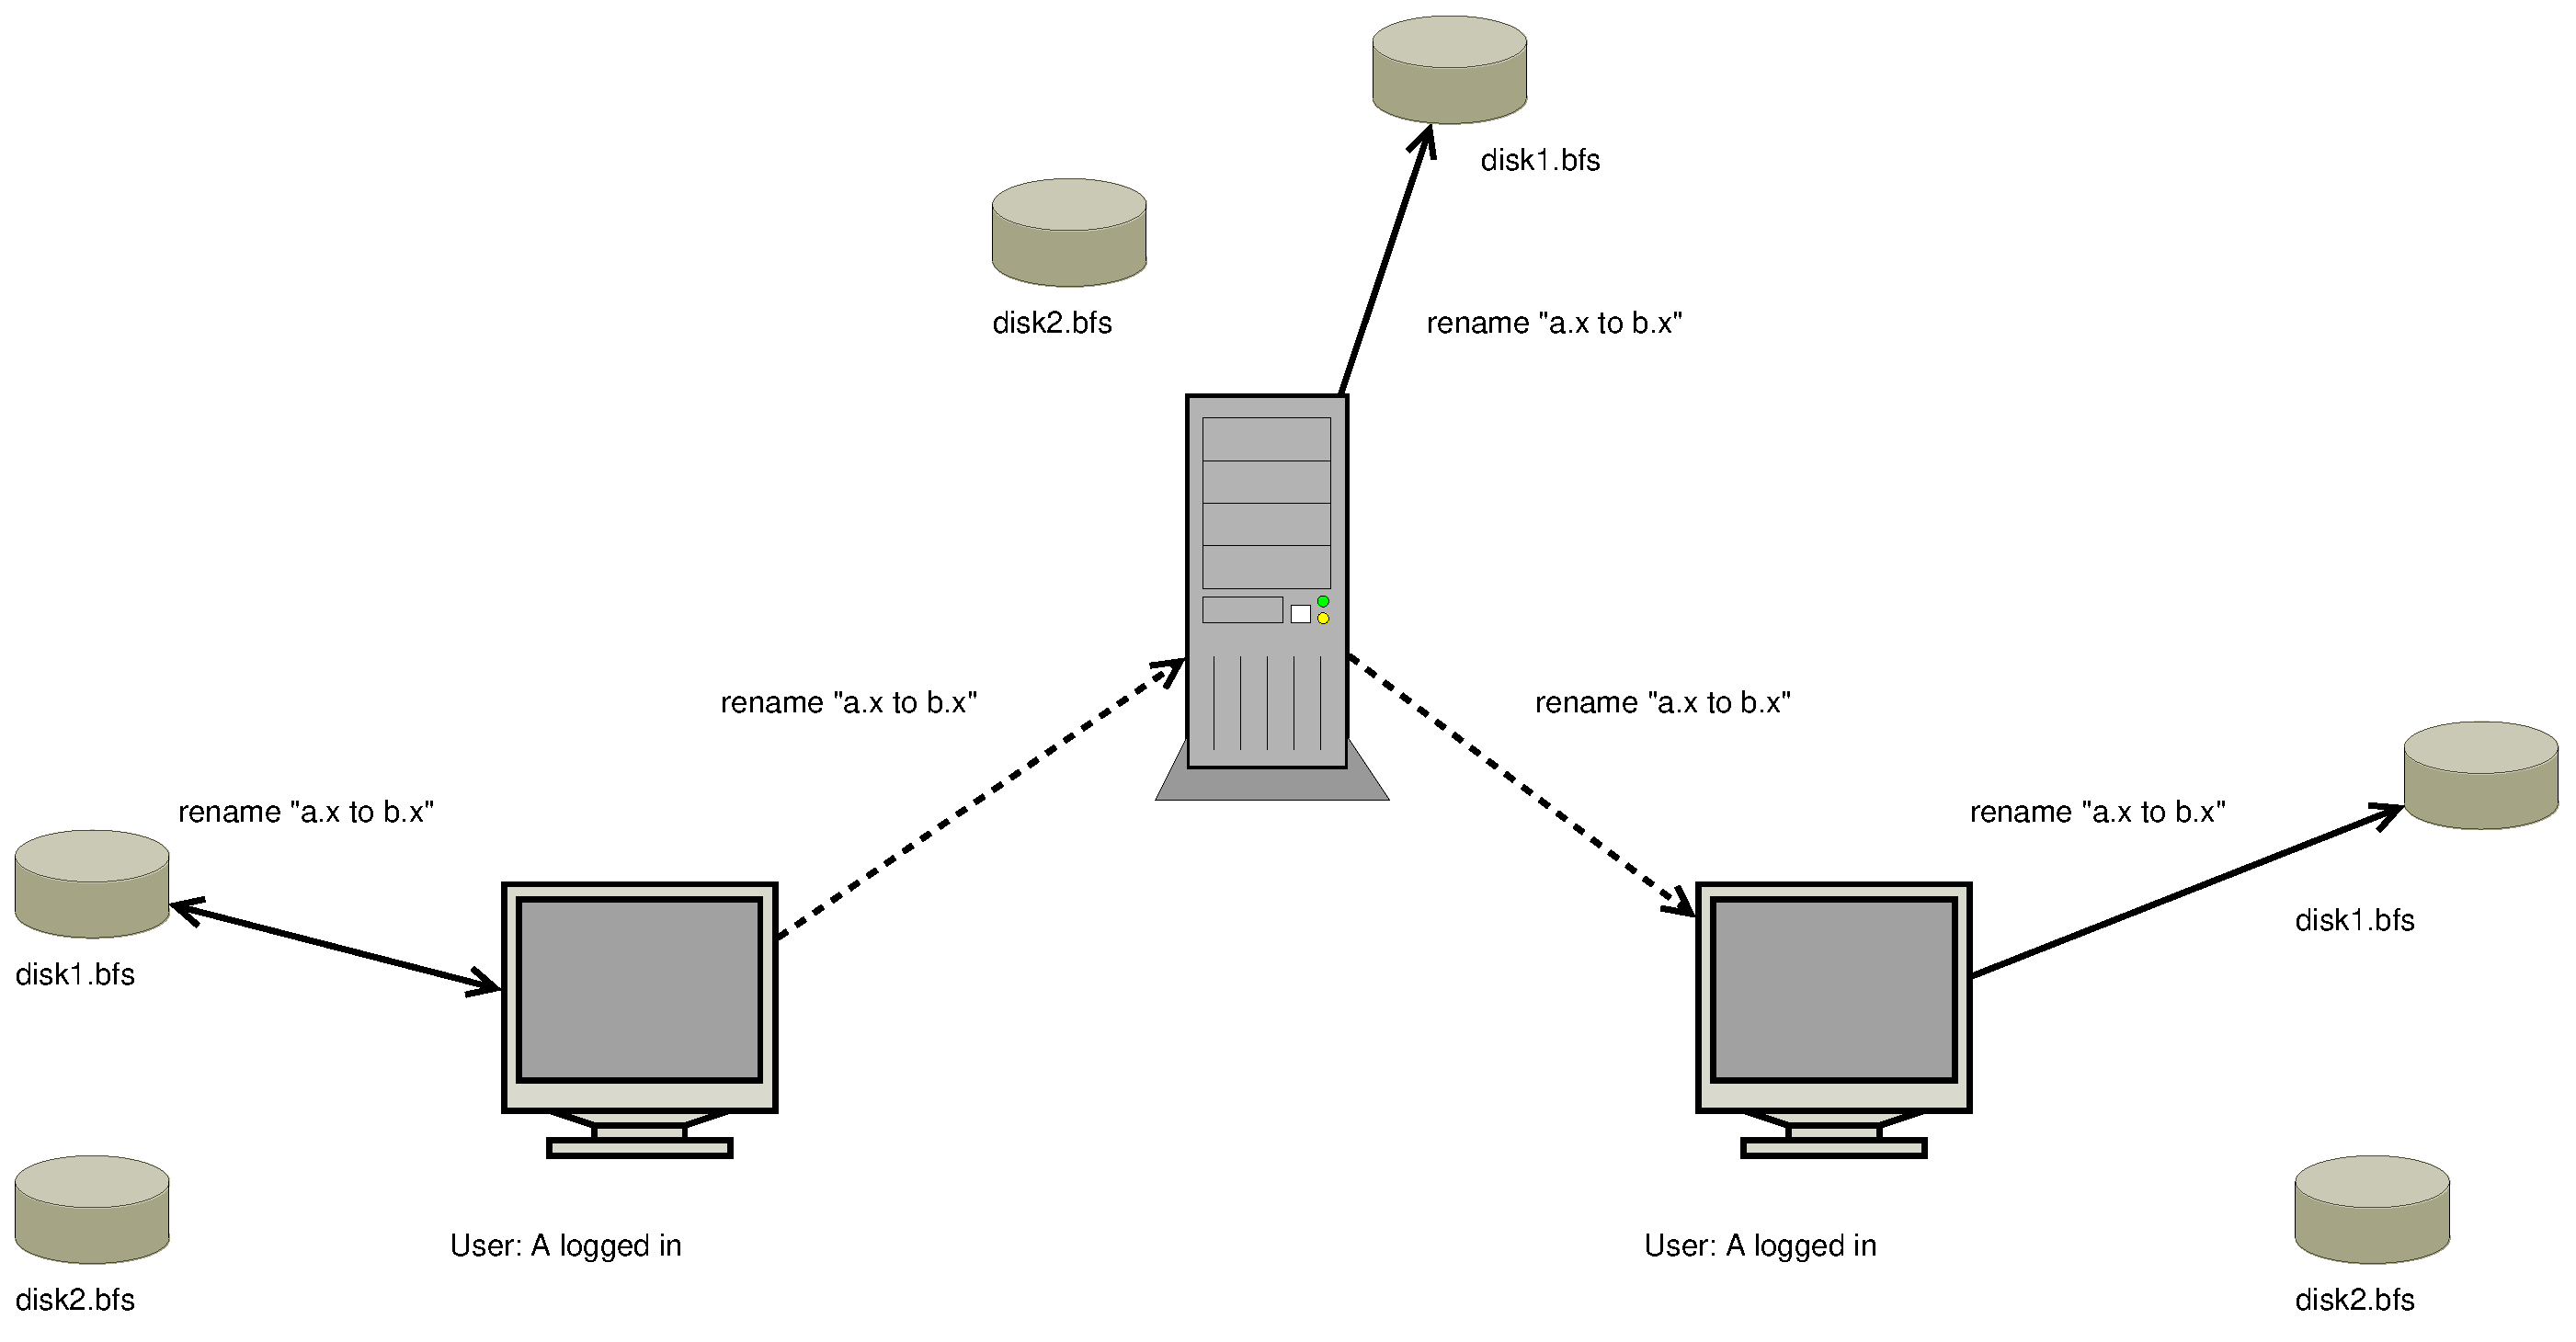
\includegraphics[width=1\textwidth]{figures/scenario_online_mode.eps}
\caption{scenario online mode}
\label{fig:scenario_online_mode}
\end{figure}

\paragraph{offline mode}

\begin{figure}[h!]
\centering
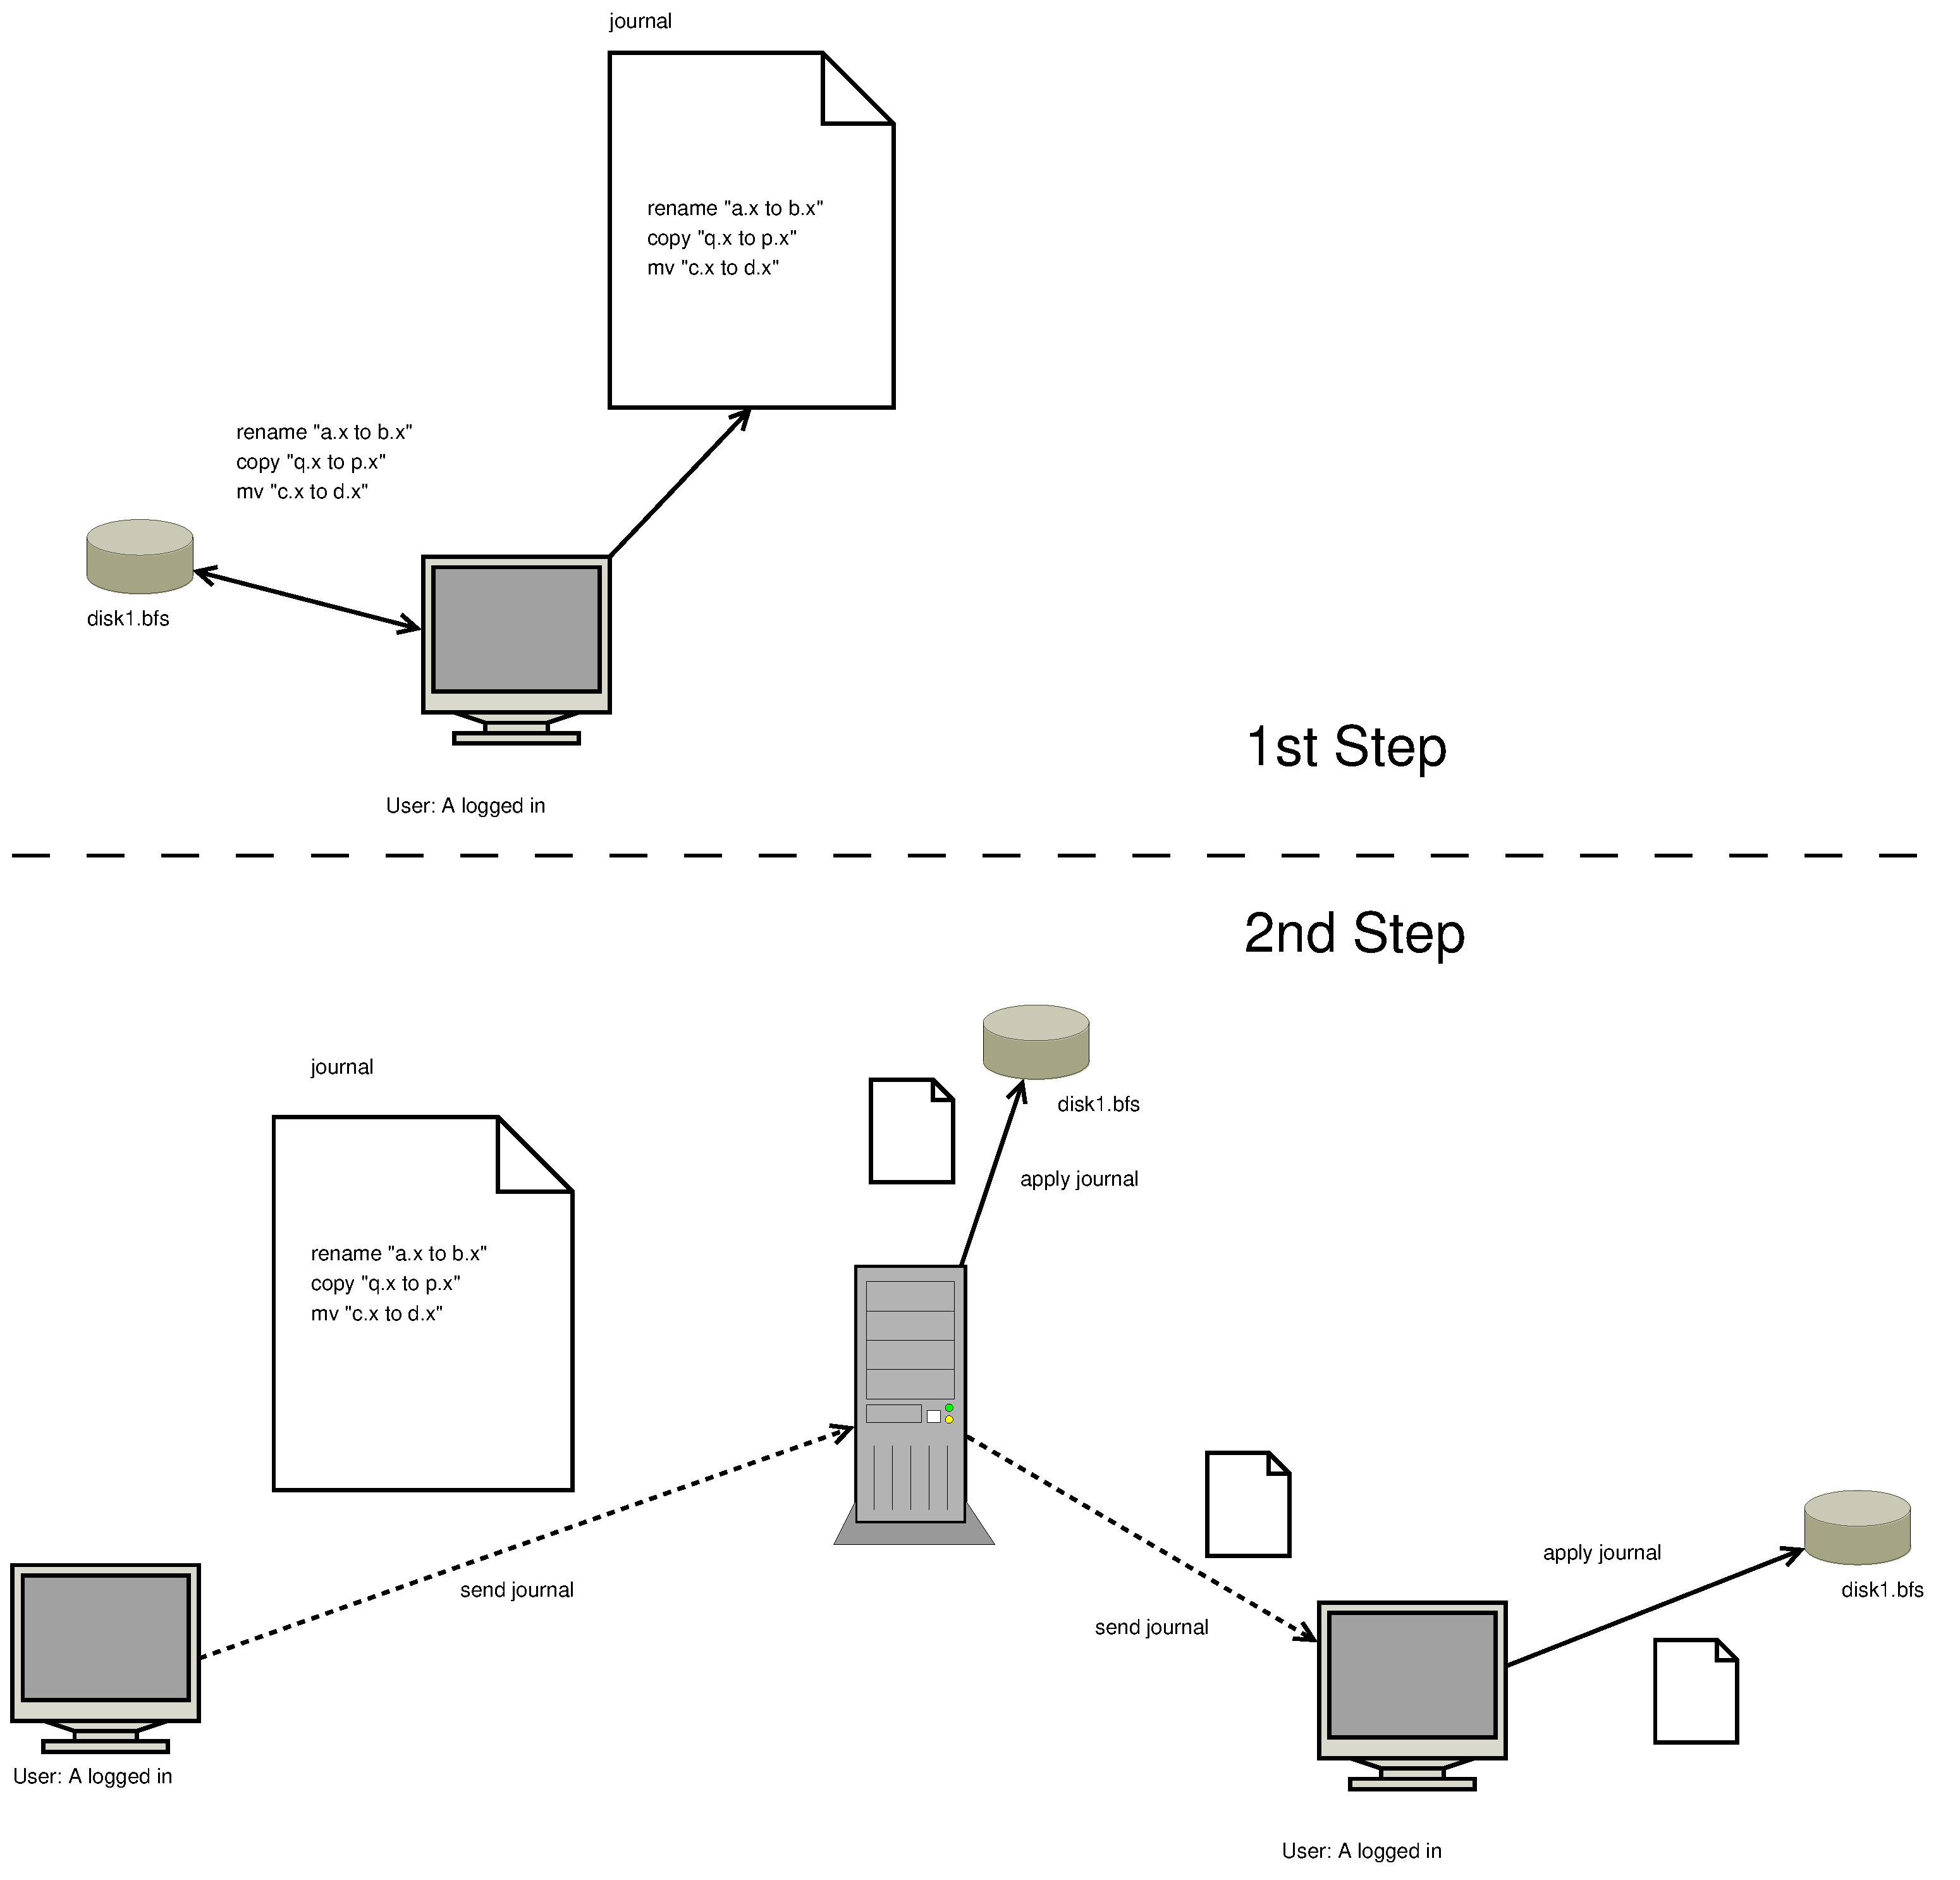
\includegraphics[width=1\textwidth]{figures/scenario_offline_mode.eps}
\caption{scenario offline mode}
\label{fig:scenario_offline_mode}
\end{figure}

\subsubsection{Technology}
RMI and so
\subsubsection{User Management}
\subsubsection{Synchronization}


Journaling

longterm polling

Schwierigkeiten mit single threaded access auf disk, auswirkungen auf das gui bei leseaktionen aka change folder


wie funktionieriert upload/download

Sequenzdiagrämmli
\paragraph{Upload changes}


\begin{figure}[h!]
\centering
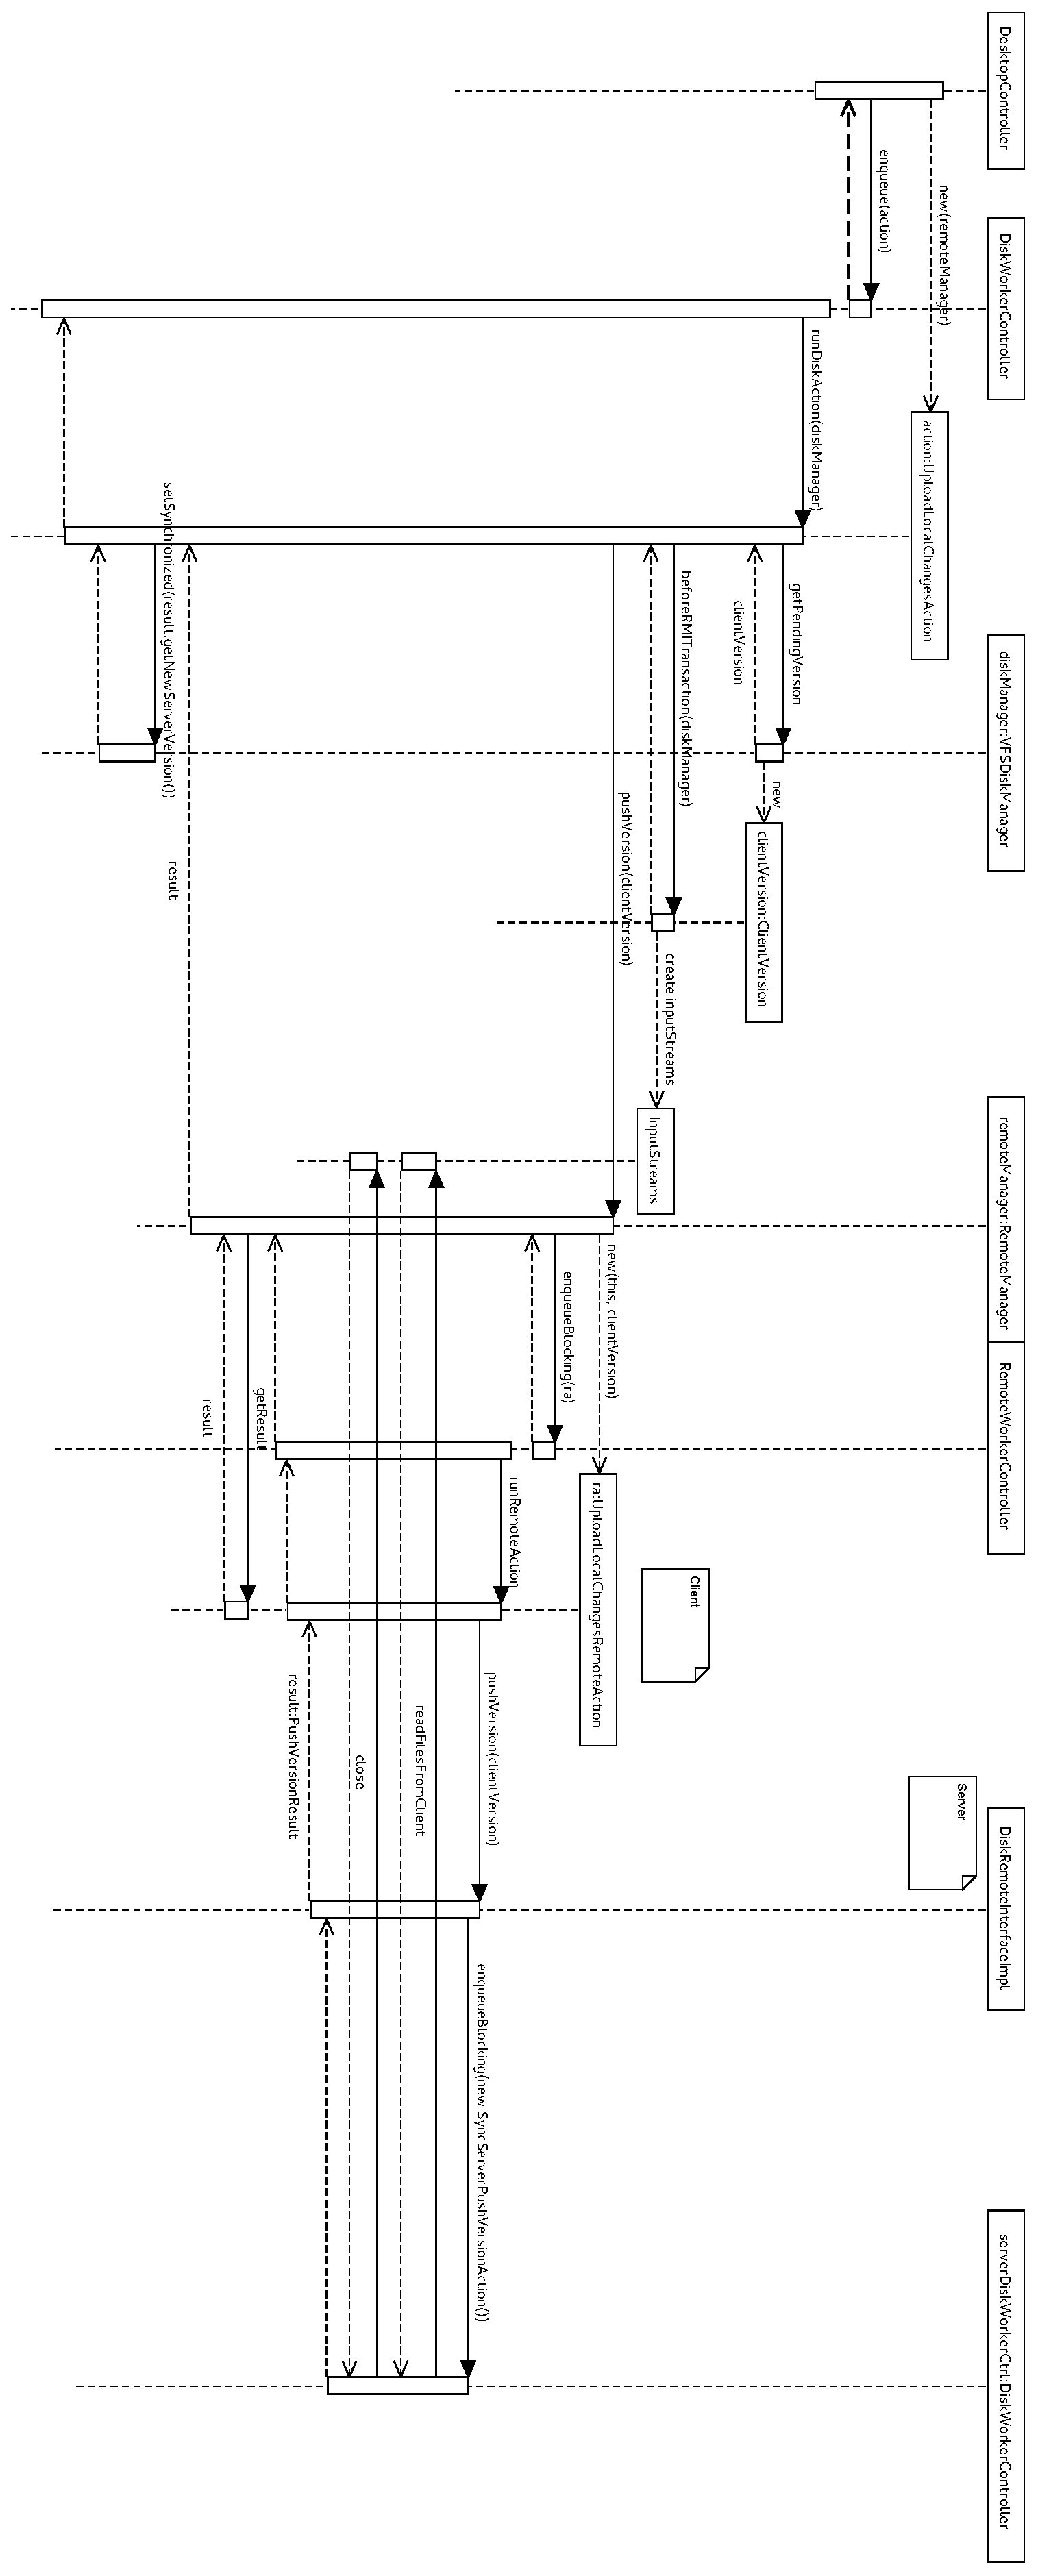
\includegraphics[height=\textheight,width=\textwidth,keepaspectratio]{figures/22uploadChanges.eps}
\caption{from click to upload changes to server}
\label{fig:uploadChanges}
\end{figure}


\paragraph{download changes}
\begin{figure}[h!]
\centering
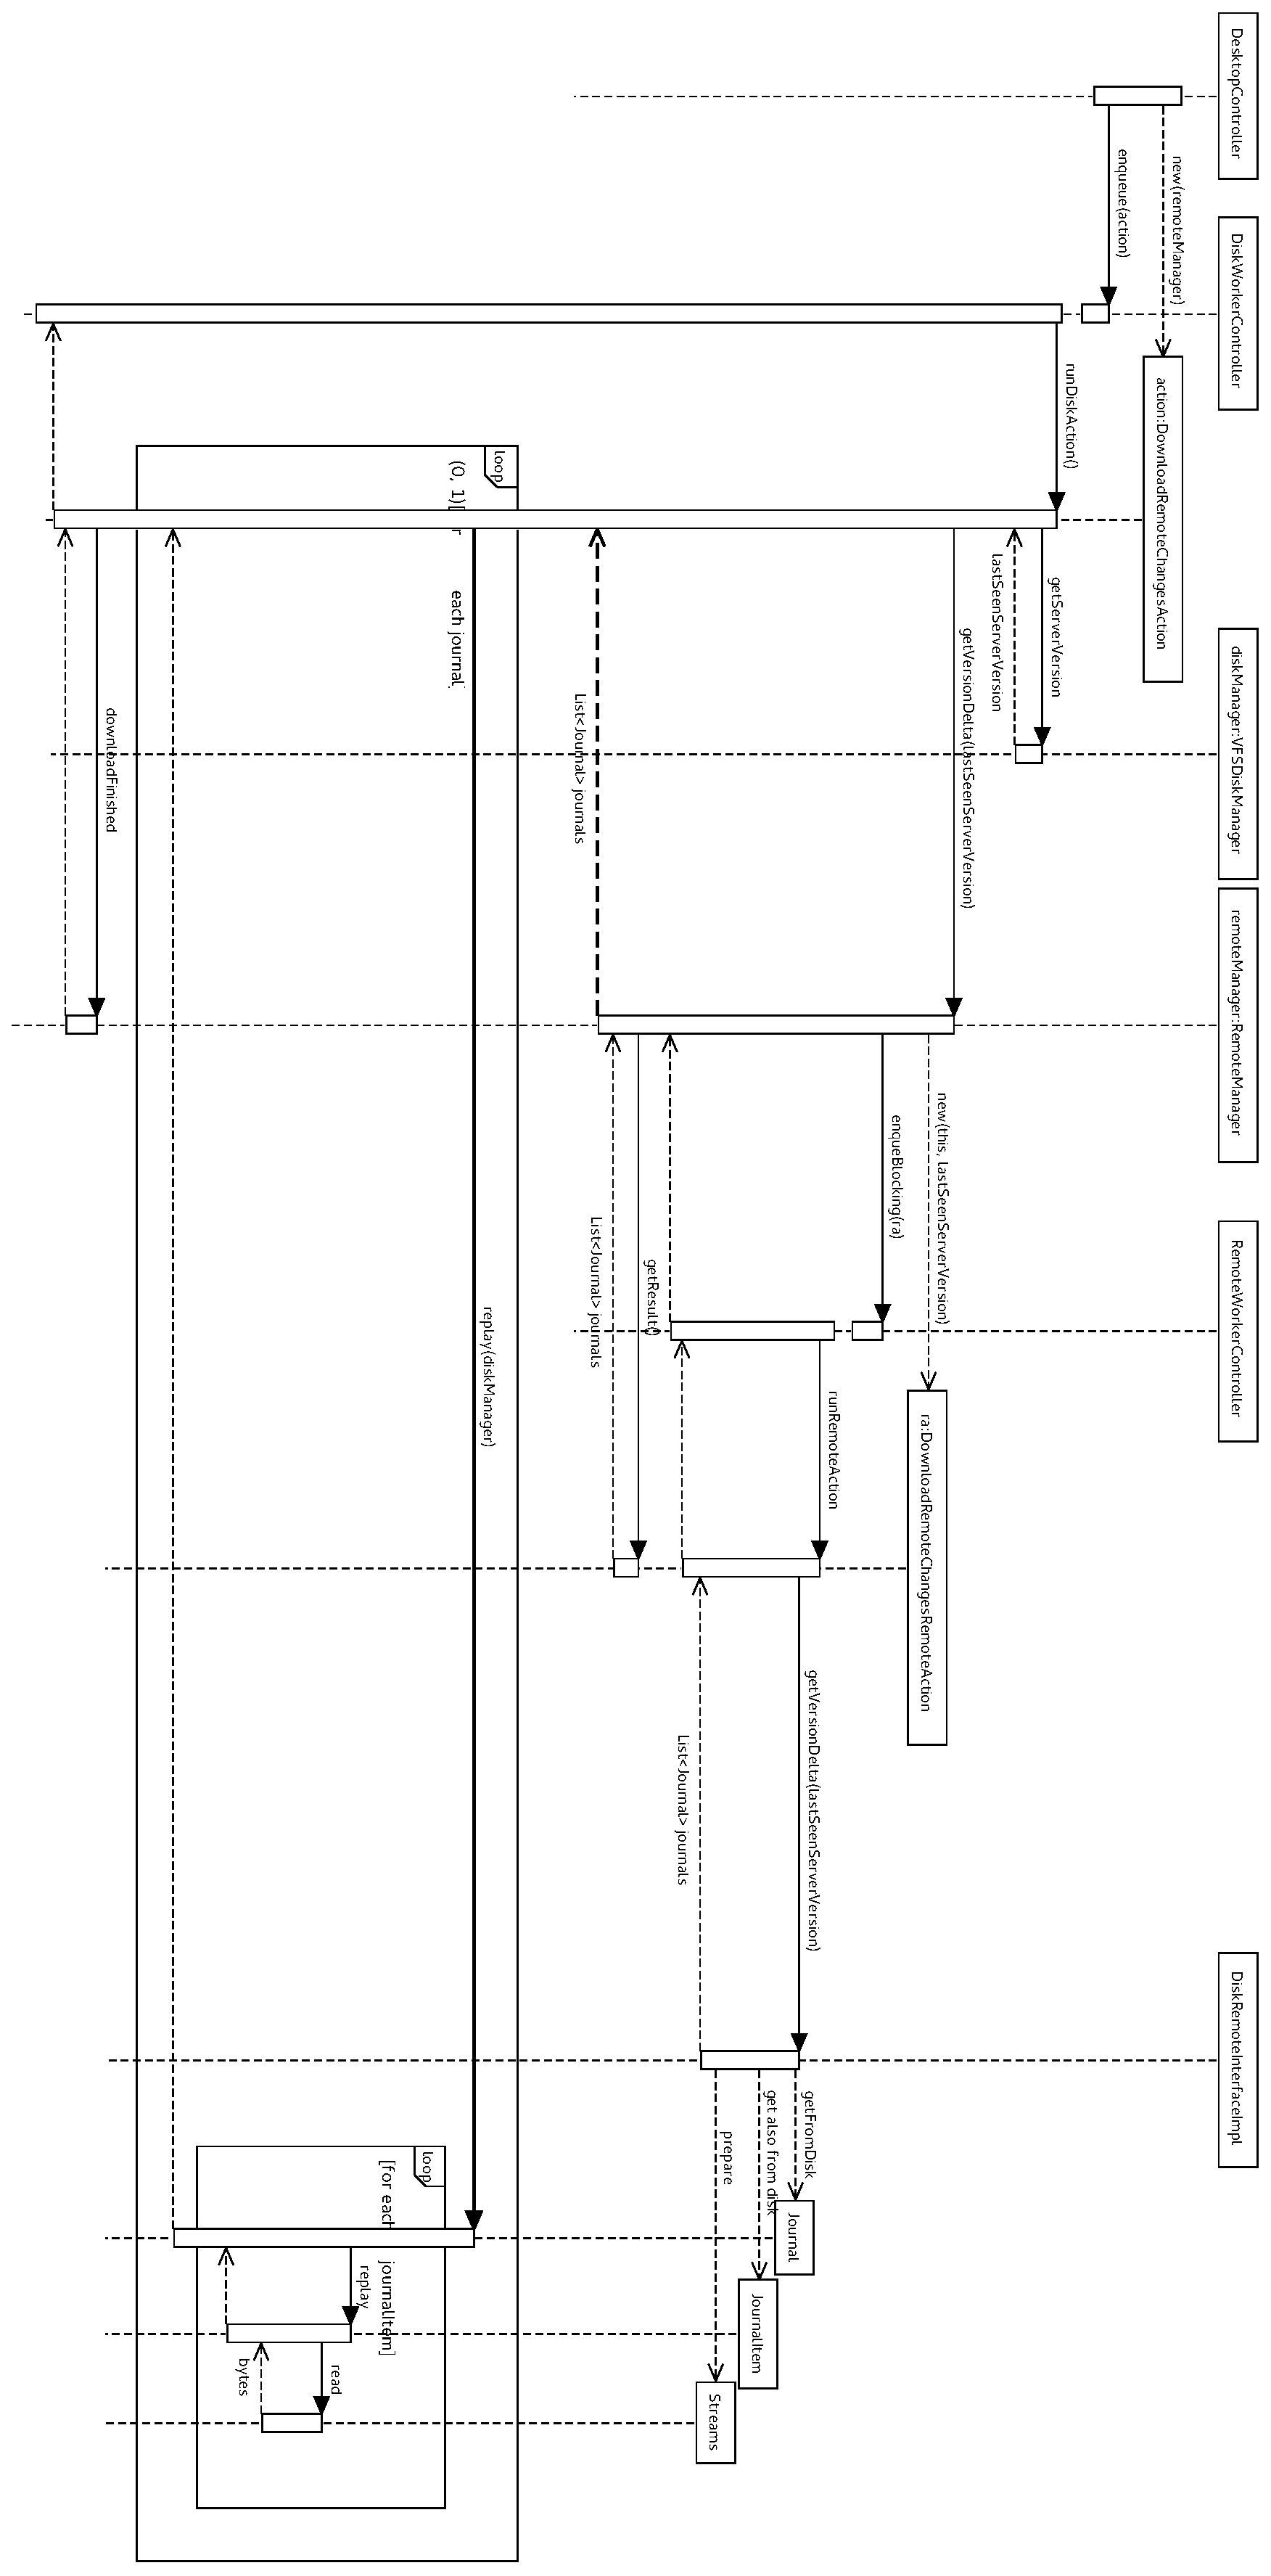
\includegraphics[height=\textheight,width=\textwidth,keepaspectratio]{figures/22downloadChanges.eps}
\caption{from click to download changes from server}
\label{fig:downloadChanges}
\end{figure}

 fancy shallow copy of files